\chapter{Revenue}

\section{Overview}

\paragraph{} As stated in the Goals section of the Overview chapter, one of the goals of OpenCombat is to develop alternative financing models such that the development of this and other games can be sustained without the need for venture capital. Although selling ownership of a game or the company that develops it does not inherently impact the development process in a negative way, the interests of venture capitalists may not always align with the interests of players or the developers themselves. This can result in products being shipped before they are ready, an over-reliance on microtransactions and other issues that can often lead to a game's decline. The philosophy behind financing and marketing OpenCombat is that revenue is derived from a quality experience not that the experience should be designed to generate revenue.

\section{The State of Revenue in Media}

\paragraph{} Currently, the highest-grossing franchises largely make their revenue from merchandising. This includes the sale of shirts, figures and similar commodities that can be used to express a consumer's interest in the franchise. Although some franchises do make substantial revenue from the original source media (games, movies, books, etc.), the vast majority is derived from the sale of merchandise. For this to be a meaningful source of funding for OpenCombat, the intellectual property must be compelling enough for players to be invested in expressing their interest publicly.

\pagebreak

\begin{figure}[h!]
    \centering
    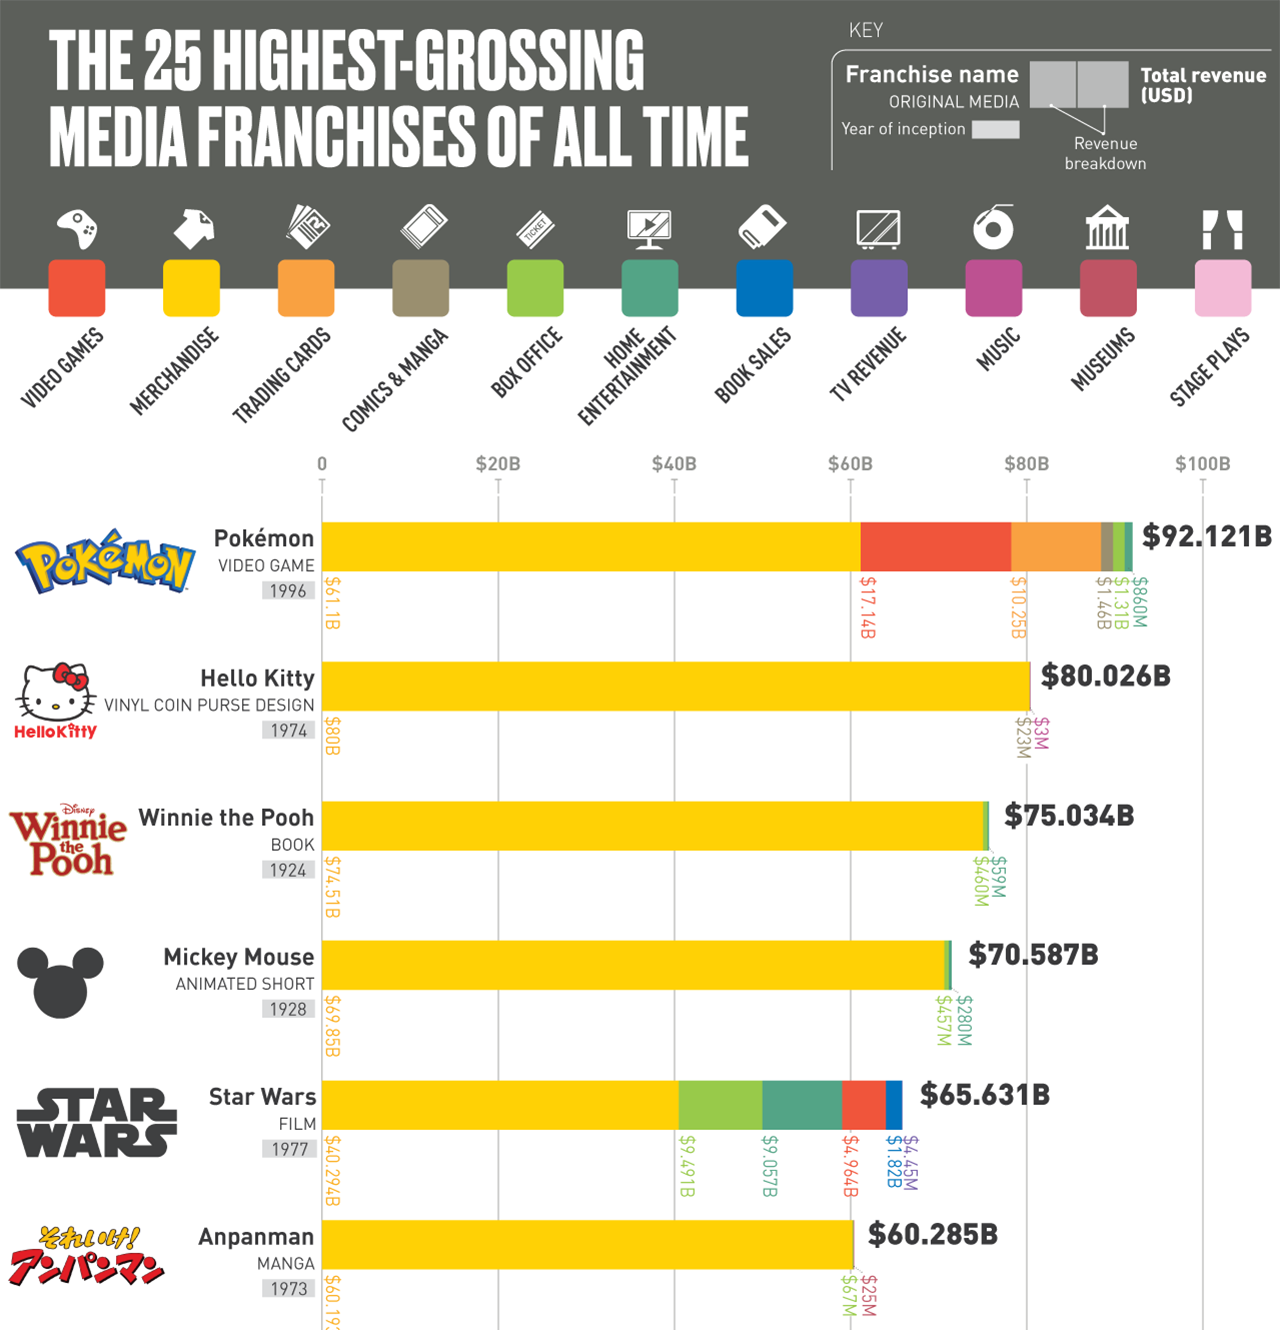
\includegraphics[width=1\linewidth]{images/highest-grossing-media-franchises-all-time.png}
    \caption{The highest grossing media franchises broken down by sources of revenue.\nocite{titlemax_top_nodate}}
\end{figure}

\pagebreak

\section{Merchandising}

\paragraph{} As previously stated, merchandising is the primary source of revenue for media franchises. In order to effectively profit from this, the intellectual property and experience of the game must be compelling enough for players to have a personal investment in the game. To encourage players to purchase merchandise, all of it will be fair trade. Although this will make the products more expensive, it also gives players a sense that their purchase is socially-conscience. Merchandise can be created to reflect the intellectual property of the vanilla experience, any additional content added through updates, inside jokes and memes from the community as well as promotions for charity drives and other community events. People will be able to purchase the merchandise from an online store owned and maintained by the company that develops OpenCombat. The game's community experience pool will be increased at point-of-sale; each product also has unique experience-gaining opportunities. 

\subsection{Merchandise and Community Experience Opportunities}

\paragraph{Note} The following is a list of potential merchandise and where it could be sold. This list is not exhaustive and could be expanded in the future. All opportunities are limited to one-per-item-per-day.

\begin{table}[h!]
    \centering
    \begin{tabular}{|c|l|}
        \hline
        \textbf{Items} & \multicolumn{1}{|c|}{\textbf{Additional Community Experience Opportunities}}\\
        \hline
        Clothing & Scan someone else wearing merchandise in public and have them confirm the scan.\\
        \hline
        Food & Scan the QR code on individual food items before consumption.\\
        \hline
        Collectables & Scan the QR code on individual collectables.\\
        \hline
        Table-Top RPG & The game master can scan a QR code on the book and have all their players confirm the session.\\
        \hline
        Music & Listen to a complete track from start to finish on the company's website.\\
        \hline
        Kitchenware & Scan the QR code on the product which can only be exposed by food or drinks.\\
        \hline
        Accessories & Scan someone else wearing or using the accessory and have them confirm the scan.\\
        \hline
        Adult Toys & Scan QR code on the toy and have all partners confirm use if applicable.\\
        \hline
    \end{tabular}
\end{table}

\section{Patreon Donations}

\paragraph{} Players will have the option to contribute to the development of the game by donating money through the web service Patreon. Through the service, donors can be rewarded with special merchandise and in-game badges that they can optionally display on their profile. Players will have access to the Patreon link through the game itself, the company website and all social media platforms.

\pagebreak

\section{Community Event Drives}

\paragraph{} Large-scale events such as charity drives and eSports tournaments are commonplace in gaming today. OpenCombat can help these events by providing support or special builds of the game in-exchange for donation pushes. For charity events in particular, the company that develops OpenCombat can encourage people to donate by giving the share of the revenue to a particular organization or cause.

\begin{table}[h!]
    \centering
    \begin{tabular}{|c|c|}
        \hline
        \multicolumn{2}{|c|}{\textbf{Current Events}}\\
        \hline
        \textbf{eSports} & \textbf{Charity} \\
        \hline
        EVO & Games Done Quick\\
        \hline
        Apex & Extra Life\\
        \hline
        Genesis & \\
        \hline
        Frostbite & \\
        \hline
        SmashCon & \\
        \hline
        Dreamhack & \\
        \hline
        Pound & \\
        \hline
        CEO & \\
        \hline
        The Big House & \\
        \hline
        Shine & \\
        \hline
        Smash n' Splash & \\
        \hline
        Get On My Level & \\
        \hline
        Low Tier City & \\
        \hline
    \end{tabular}
\end{table}